A continuación se procede a explicar las pruebas realizadas en cada una de las áreas mencionadas anteriormente

\subsection{Pruebas en el diseño de las piezas 3D}
\

Desde los momentos iniciales del proceso de impresión se observa que ciertas partes de las piezas impresas no concuerdan en tamaño con el especificado en el diseño 3D. Este problema se hace evidente en las características que requieren de alta precisión como pueden ser los agujeros para los tornillos o los dientes de los engranajes.

Dado que existe esta diferencia entre el tamaño real y el tamaño del diseño, el equipo de desarrollo realiza varias pruebas para determinar que tamaño es necesario definir en el diseño para que, al imprimir, se obtenga el tamaño deseado.

Estas pruebas se han tenido que hacer para determinar el tamaño necesario para los tornillos de métrica 3 y 4 además de los ejes y los rodamientos.

Las pruebas consisten en imprimir una piezas con varios agujeros de diámetros variables con el objetivo de averiguar que tamaño es el adecuado.

A continuación se pueden observar dichas piezas.

\begin{figure}[H]
    \centering
    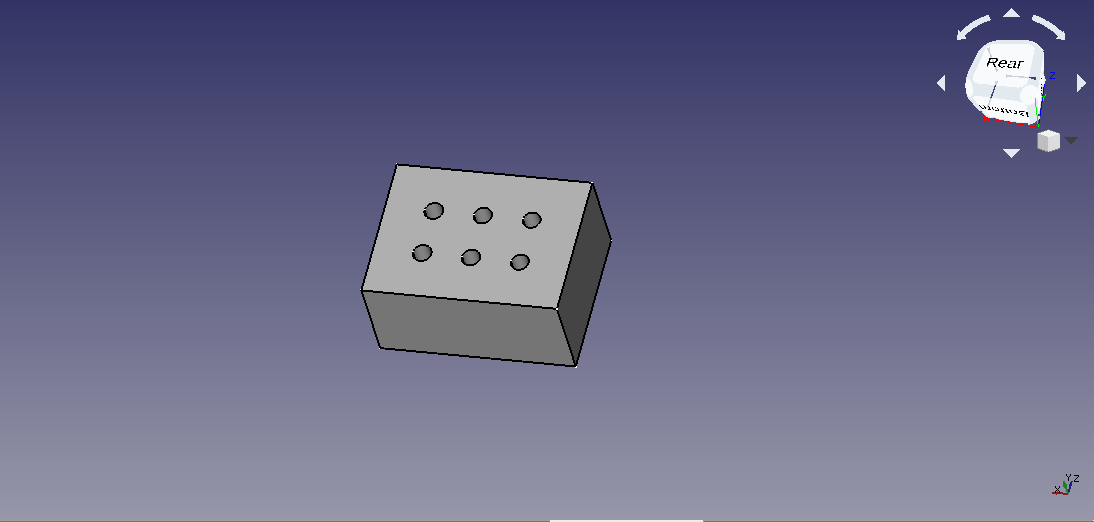
\includegraphics[width=.7\linewidth]{pictures/LadrilloPrueba.png}
    \caption{Pieza de prueba para tornillos M4}
    \label{fig:prueba_m4}
\end{figure}

\begin{figure}[H]
    \centering
    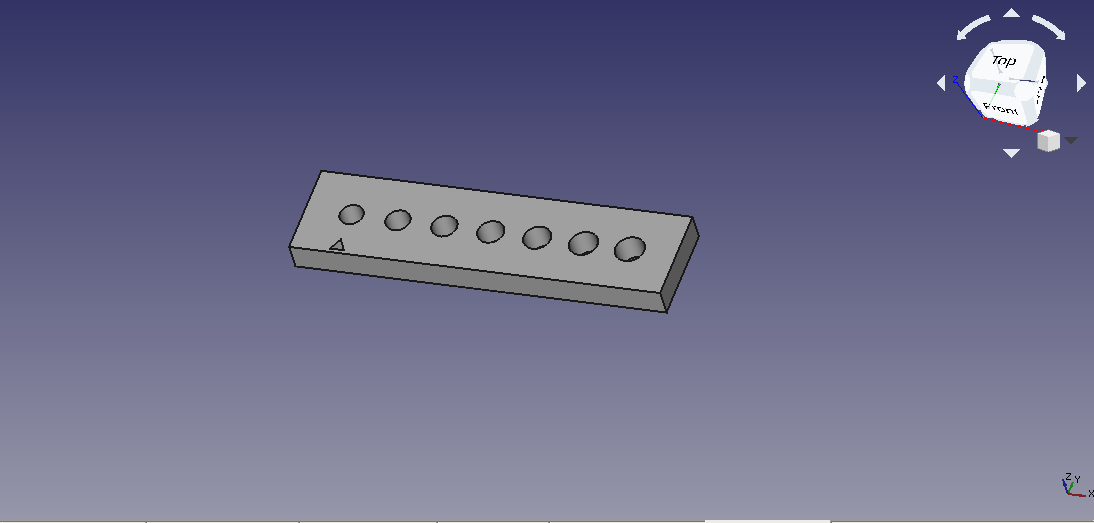
\includegraphics[width=.7\linewidth]{pictures/PruebaM3.png}
    \caption{Pieza de prueba para tornillos M3}
    \label{fig:prueba_m3}
\end{figure}

\begin{figure}[H]
    \centering
    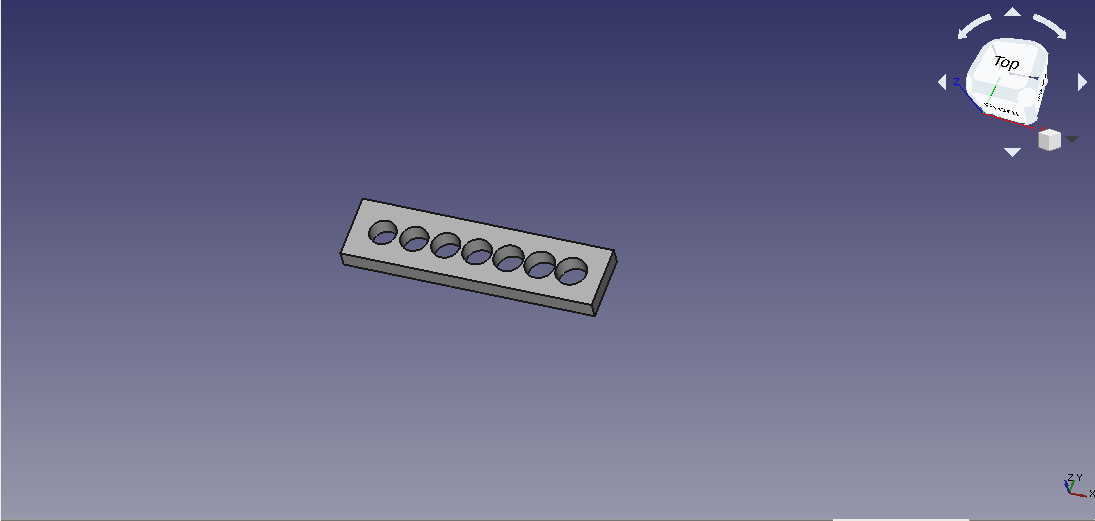
\includegraphics[width=.7\linewidth]{pictures/PruebaEje.png}
    \caption{Pieza de prueba para eje de 4 mm de diámetro}
    \label{fig:prueba_eje}
\end{figure}

Tras realizar estas pruebas se tomaron las siguientes decisiones técnicas.

Para tornillos de métrica 3 (véase figura \ref{fig:prueba_m3}) el agujero del diseño 3D deberá tener 2,8mm de diámetro. Con este diámetro se consigue suficiente material adicional en las paredes del agujero para que tras introducir el macho quede una rosca suficientemente profunda.

Para diámetros menores, el macho no podía ser introducido en el agujero y por tanto no se podía hacer rosca,

Para diámetros mayores, el macho entraba con demasiada holgura o bien no había suficiente material adicionar para crear una rosca resistente.

Es necesario recordar que el tornillo es metálico y el agujero es plástico por lo que una rosca resistente es necesaria debido al desgaste que el tornillo ejerce sobre el plástico.

Para tornillos de métrica 4 (véase figura \ref{fig:prueba_m4}) el agujero del diseño 3D deberá tener 3,8mm de diámetro. Las razones son las mismas que las expuestas anteriormente para el tornillo de métrica 3.

En el caso de los ejes se siguió una metodología similar.
Para un eje de 4mm de diámetro, se debía dejar una agujero de entre 3,9 y 4,1 mm de diámetro dependiendo de la holgura que se desee.

Por otro lado, se han tenido que hacer pruebas para determinar el modulo adecuado para el engranaje exterior que transmitirá el movimiento desde el eje motor hasta las piezas que se ensamblan con el.

\begin{figure}[H]
    \centering
    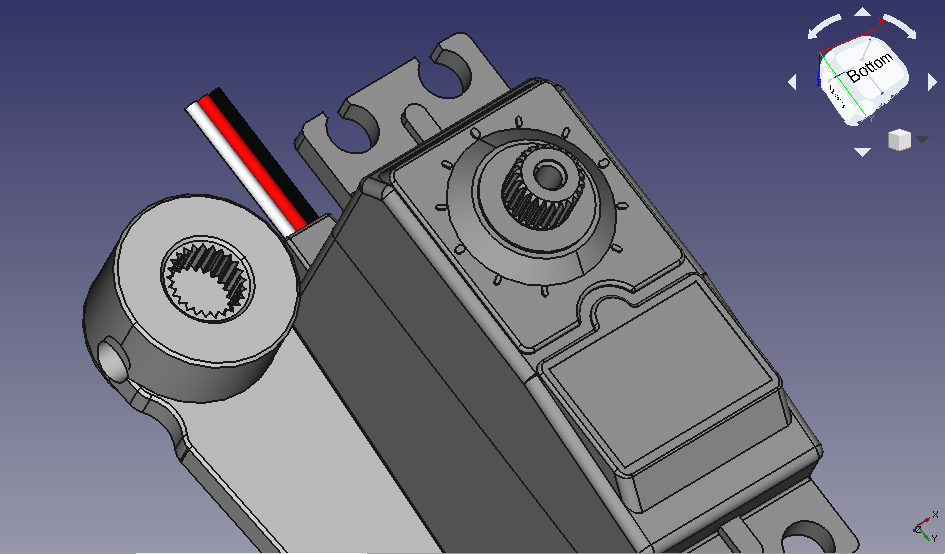
\includegraphics[width=.7\linewidth]{pictures/ComparativaEngranajes.png}
    \caption{Modelos 3D del motor empleado junto a una pieza que se ensambla en su eje}
    \label{fig:comparativa_engranajes}
\end{figure}

Como observamos en la figura \ref{fig:comparativa_engranajes} las piezas que van engranadas directamente en el eje han de tener un numero determinado de dientes y un diámetro concreto.

La cantidad de dientes viene dada por el engranaje del motor, el cual no puede ser modificado y es una restricción ajena al proceso de diseño. Sin embargo, se tuvieron que hacer pruebas para determinar el diámetro adecuado.

Tras varias pruebas se concluyo que el modulo necesario (Diámetro/Nº de Dientes) depende de si las capas que contienen los dientes son capas superiores o inferiores.
En capas inferiores el modulo ha de ser 0,257 mm mientras que en capas superiores el modulo ha de ser 0,25 mm.

Para un modulo mayor los dientes de ambos engranajes no encajaban bien y por tanto el giro no se transmitía del eje a la pieza.

Para un modulo menor el eje no entraba dentro de la pieza.

\subsection{Pruebas en la impresión 3D}

% Aqui habla de los parametros de impresón Javier.

\subsection{Pruebas post-impresión}
\label{pruebas_post_impresión}

Aprovechando ciertas piezas cuya impresión fue insatisfactoria, el equipo de desarrollo realizo pruebas destructivas para determinar el aguante ante esfuerzos de tracción, compresión y torsión.

Debido a que la estructura inferior del brazo debe soportar el peso de este, se estudio el aguante ante esfuerzos de compresión de las piezas macizas donde se concluyo que pueden aguantar pesos superiores a 50Kg sin deformarse.

Por otro lado, el esfuerzo de tracción se ha estudiado al completar la estructura del brazo, y se ha concluido que las piezas son capaces de soportar, al menos, el propio peso de la estructura.

%El esfuerzo de torsión ha sido estudiado sobre las piezas que han de transferir el movimiento desde el eje motor hasta la estructura. También se ha concluido que será capaz de soportar al menos el propio peso de la estructura.%

Cabe destacar que en las piezas que son atravesadas por tornillos, se han observado problemas en las roscas de poca profundidad. Al ser el acero un material mucho mas duro que el plástico, este puede romper los surcos de las roscas de plástico si estas son muy superficiales, ya que el esfuerzo se realiza sobre un numero mas reducido de surcos que en el caso de una rosca mas profunda. 

Concretamente este problema aparece en las piezas que tienen tornillos para hacer presión sobre el eje.

Para solucionar este problema se ha decidido limar el eje en las zonas donde este entre en contacto con los tornillos, de esta manera la fuerza que se ha de ejercer para mantener el eje fijo es menor y por tanto no se fuerzan las roscas.